
\chapter{HTR Model} 
\label{ch:Chapter5}
\vfill \minitoc \newpage

\section{Introduction}
Handwriting recognition \gls{htr} is a technology that converts handwritten text into digital format. Its purpose is to enable the efficient processing, storage, and manipulation of handwritten content through automated recognition algorithms.

\subsection{Offline HTR}
Offline handwriting recognition refers to the technology and process of converting static images or scans of handwritten text into digital text or characters. Unlike online handwriting recognition, which interprets handwriting in real time as it is being written, Offline \gls{htr} analyzes pre-existing images or documents that have been captured or scanned.

The goal of Offline \gls{htr} is to accurately recognize and convert the handwritten text in images into editable and searchable digital format. This technology finds applications in digitizing historical documents, handwritten notes, forms, and any other handwritten content that needs to be converted into machine-readable text.

The process of Offline \gls{htr} typically involves several steps:
\begin{itemize}
    \item Detection: In the detection phase, the handwritten text regions within the scanned or captured images are identified. This can be achieved through techniques such as text detection algorithms, connected component analysis, or contour-based methods. The goal is to localize and extract the regions containing the handwritten content for further processing.

    \item Image preprocessing: The scanned or captured images are enhanced, filtered, and prepared to optimize the quality of the handwriting for recognition. This may involve noise reduction, binarization, deskewing, and other techniques.
    
    \item Recognition: Machine learning algorithms, such as neural networks or Hidden Markov Models (HMM), are trained using labeled samples of handwritten characters or words. These models are then used to recognize and classify the extracted features into corresponding textual representations.

    \item Post-processing: The recognized text is further refined and processed to improve accuracy, correct errors, handle ambiguities, and align with language-specific rules and dictionaries.

\end{itemize}


\subsection{Online HTR}
Online handwriting recognition refers to the technology and process of converting handwritten input into digital text or characters in real time. It involves capturing and interpreting the movements and patterns made by a user while writing using a stylus or a digital pen on a touch-enabled device, such as a tablet or a smartphone.

Unlike offline handwriting recognition, which analyzes static images of handwritten text, online handwriting recognition takes advantage of the temporal information obtained during the writing process. This allows for real-time interpretation and immediate feedback as the user writes, making it suitable for applications where instant recognition is required, such as note-taking, electronic signature verification, form filling, and interactive whiteboards.

Online handwriting \textit{\cite{OnlineHTR}} recognition systems typically use various techniques, including pattern recognition algorithms, machine learning, and neural networks, to analyze the dynamic information provided by the user's pen strokes. These algorithms analyze factors such as stroke speed, direction, pressure, and sequence to identify and interpret the handwritten characters or gestures. The recognized text can then be further processed, stored, or used in various applications and systems that require digital text input.


\section{Implementation}
In this section we will talk about the decisions made and explain the implementation of each component.
\subsection{Why Offline HTR}
In a project like this, it initially seems like a no-brainer to implement Online \gls{htr} instead of Offline \gls{htr}. However, the lack of complex yet comprehensive documentation for beginners pose a significant roadblock. Without readily available resources and clear guidance, the implementation process becomes more complex and time-consuming. This led to frustration and delays as the we struggled to navigate the complexities of Online \gls{htr} without proper guidance.

Furthermore, the absence of open-source implementations of Online \gls{htr} hinders collaboration and knowledge sharing within the community. Open-source projects often serve as valuable starting points, providing code samples, libraries, and frameworks that accelerate the development process. Without such resources, we must start from scratch or rely on proprietary solutions, limiting the ability to customize and adapt the \gls{htr} system to the specific project requirements. The potential benefits of enhanced accuracy,  real time text recognition, and dynamic input support opportunities may be overshadowed by the steep learning curve and lack of accessible resources for offline \gls{htr} implementation.

As a result, the decision to implement Offline \gls{htr} becomes less straightforward yet possible thanks to widely available open-source implementations and good guidance examples such as the one followed to implement our model \textit{\cite{HTR}}.


\subsection{Pipeline}
The \gls{htr} system follows a pipeline-based approach to process images and extract text. The pipeline consists of two main stages: text detection and text recognition.
The Figure~\ref{fig:HTRS} represents a overview of the implemented \gls{htr} system. For our needs it takes a PNG containing the postcard drawn content and returns the text as a String. 

\begin{figure}[!ht]
	\centering
	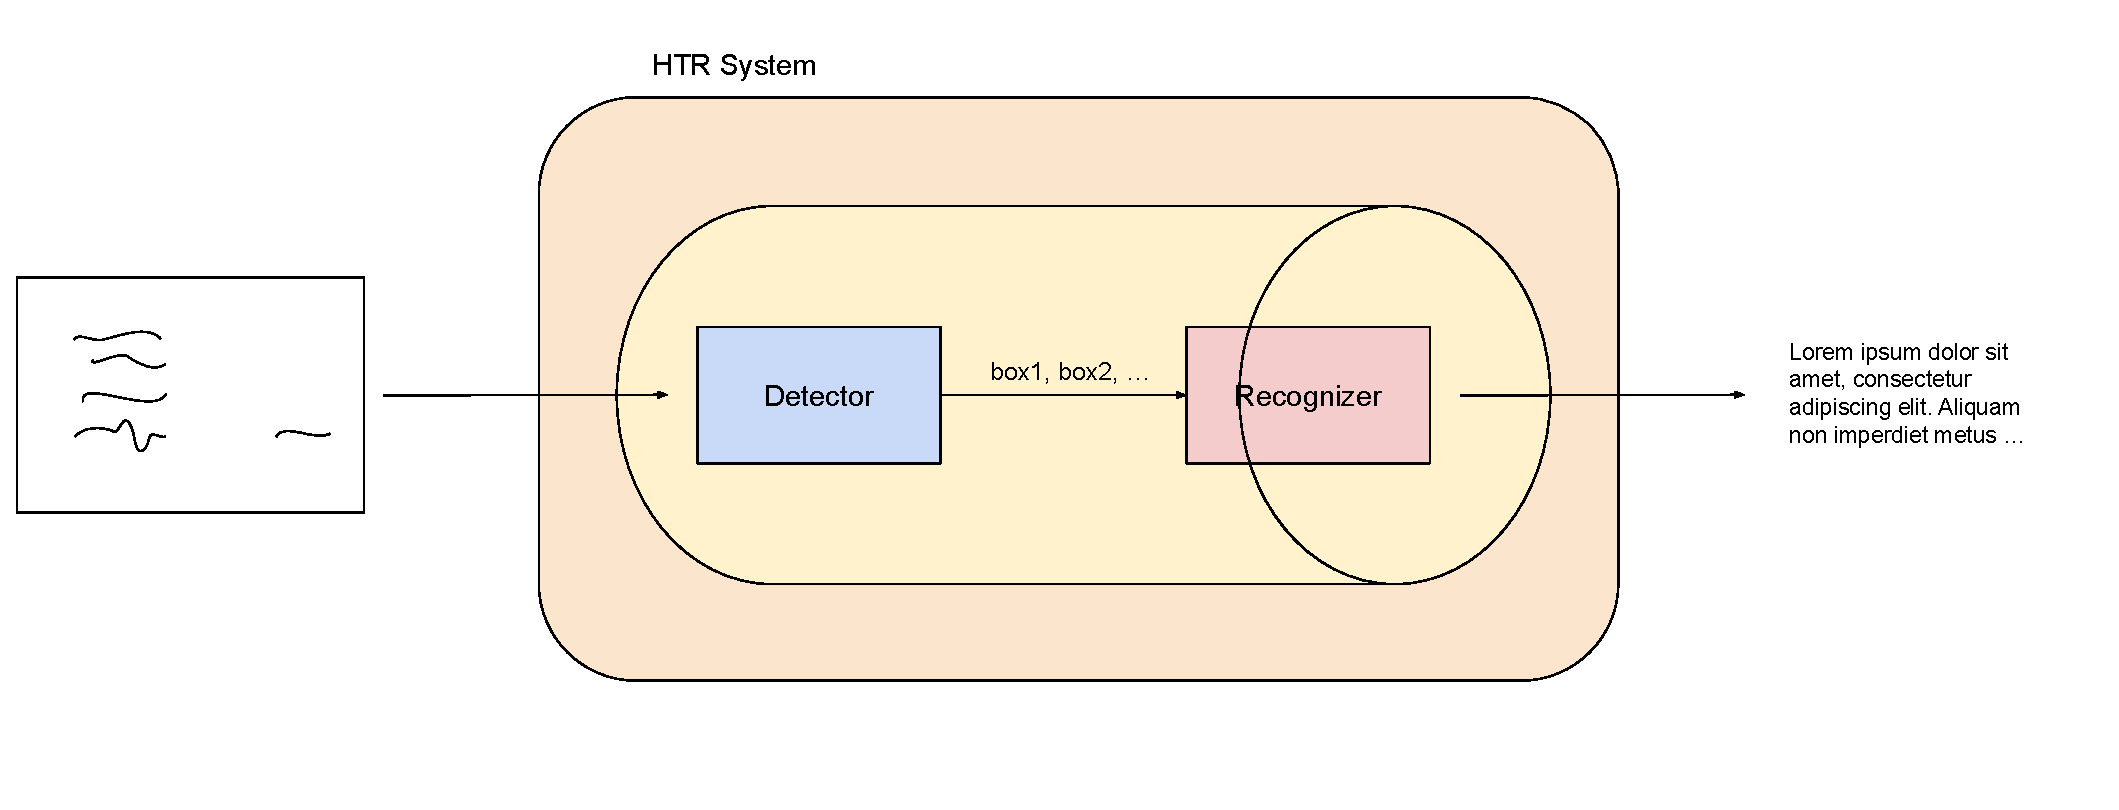
\includegraphics[trim={ 0.2cm 1cm 0cm 0cm },width=1\textwidth]{./Chapter5/Figures/HTR System}
	\caption{HTR System}
	\label{fig:HTRS}
\end{figure}

\textbf{Both components use the Tensorflow framework and are written in python.}

\subsection{Detector}
The detection is made possible by using CRAFT-Text \textit{\cite{CRAFT-Text}} detection implementation from \textit{\cite{Keras-ocr}}. The particular detector was trained for machine-generated characters based on fonts but still manages to give good results for handwritten text, big part of it's good results is the absence of visual clutter in the background as we only provide the drawn content to the model. 


The Figure~\ref{fig:Detector} illustrates how the detector works, keeping in mind that the figure is simplified for explanatory purposes and the detector detects words and not lines.

\begin{figure}[!ht]
	\centering
	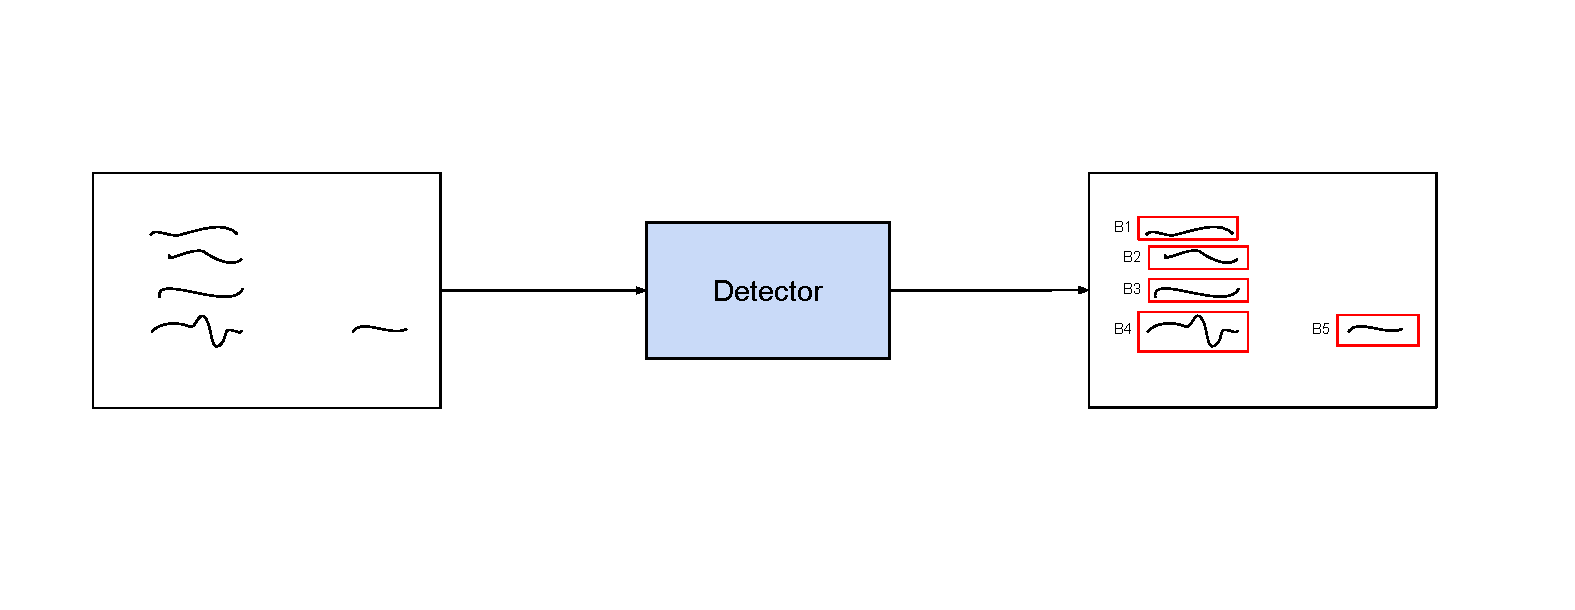
\includegraphics[trim={2cm 3cm 0 1cm}, width=1.1\textwidth]{./Chapter5/Figures/Detector}
	\caption{Detection Flow}
	\label{fig:Detector}
\end{figure}

The returned value from the detector model is a list containing four points (x and y) defining a box that represents where the word is relative to the image.


\subsection{Recognizer}
The text recognition stage takes the boxes from the detector and processes them to extract the actual text content creating a temporary file for each box. It applies character segmentation, feature extraction, and sequence modeling techniques to recognize and convert the text regions into machine-readable format. A layer by layer summary based on online documentation:
\begin{itemize}
    \item Input Layer: The model takes an input image with dimensions (128, 32, 1), representing a grayscale image. It also takes input labels, which are sequences of characters.
    \item Convolutional Layers: The model starts with two convolutional blocks. Each block consists of a 2D convolutional layer followed by a max-pooling layer. The convolutional layers learn local image features and the max-pooling layers downsample the feature maps.
    \item Reshaping and Dense Layer: After the convolutional layers, the feature maps are reshaped to a new shape that is compatible with the recurrent part of the model. This reshaping operation prepares the data for input to the recurrent layers. The reshaped features pass through a fully connected dense layer with 64 units and ReLU activation.
    \item Dropout Regularization: A dropout layer is applied to reduce overfitting by randomly setting a fraction of the input units to 0 during training.
    \item Recurrent Layers: Two bidirectional LSTM layers are stacked on top of each other. Bidirectional LSTMs process the input sequence in both forward and backward directions, allowing the model to capture dependencies in both directions. The LSTM layers have dropout applied to them to prevent overfitting.
    \item Output Layer: A dense layer with a softmax activation is used as the output layer. The number of units in this layer corresponds to the vocabulary size (number of characters) plus two special tokens introduced by the CTC loss. The softmax activation produces a probability distribution over the characters.
    \item CTC Loss Layer: The output of the softmax layer is passed to the Connectionist Temporal Classification (CTC) layer. The CTC layer calculates the CTC loss, which measures the difference between the predicted sequence and the ground truth labels. It takes both the labels and the output of the softmax layer as inputs.
    \item Model Compilation: The model is compiled with the Adam optimizer. The specific learning rate and other optimizer parameters can be further customized if needed.
    \item Model Output: The output of the model is the output of the CTC layer, representing the CTC loss. 

\end{itemize}


\begin{figure}[!ht]
	\centering
	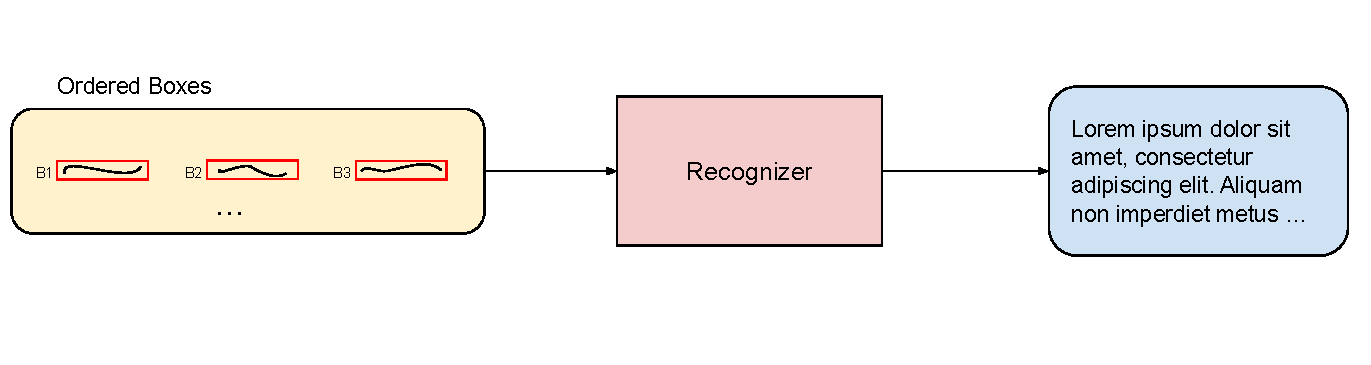
\includegraphics[trim={0cm 0cm 0 0cm}, width=1\textwidth]{./Chapter5/Figures/Recognizer}
	\caption{Recognizer Flow}
	\label{fig:Recognizer}
\end{figure}




\subsubsection{Image Preprocessing}
Image preprocessing is a critical step in offline \gls{htr} systems as it aims to enhance the quality of scanned or captured handwritten images before they are fed into the recognition model. The objective is to optimize the images for accurate recognition by applying various transformations and adjustments.

In the context of our project, the provided code snippet offers a foundational approach to image preprocessing.

Reading and Decoding Image:

The first step involves reading the image file using tf.io.read\_file and decoding it using tf.image.decode\_png.
By decoding the image as grayscale (decode\_png(image, 1)), we ensure that only the necessary information is retained.
Distortion-Free Resizing:

To achieve consistent input sizes, the distortion\_free\_resize function is employed for resizing the image to the desired dimensions (img\_size).
During resizing, the preserve\_aspect\_ratio=True parameter ensures that the original aspect ratio of the image is maintained.
This function intelligently pads the image symmetrically to ensure uniformity and prevent distortion.
Normalization:

After resizing, the image is cast to tf.float32 and normalized to a range between 0 and 1 by dividing each pixel value by 255.0.
Normalization facilitates improved convergence during training and enhances the overall performance of the recognition model.
By utilizing the preprocess\_image function, we establish a solid foundation for handling image preprocessing in our offline \gls{htr} system. This function accepts an image path as input and performs resizing, padding, and normalization operations to prepare the image for subsequent processing.


\subsubsection{Training}
The recognizer was trained using the \textit{\cite{IAM}} words dataset, which is a widely used benchmark dataset for \gls{htr} research. The IAM dataset is a comprehensive collection of handwritten English text samples contributed by different writers. It consists of 86810 training samples, 4823 validation samples and 
4823 test samples.

To get good results the recognizer was trained for roughly 60 iterations in Google's Colab Notebook servers.

\paragraph{Tweaks}
After each training iteration, the Tensorflow training process incorporates additional code through callbacks to enhance its functionality. In this particular scenario, two tweaks have been added to optimize the training process:
\begin{itemize}
    \item Early Stopping Callback:
    An early stopping callback is implemented to monitor the model's performance during training and determine if it is not improving.
    The patience parameter is set to 3, indicating that if the model does not show improvement for 3 consecutive iterations, the training process will stop early.
    By setting restore\_best\_weights to True, the callback ensures that the best weights achieved during training are restored before stopping, allowing for optimal model performance.
    The verbose parameter is set to 1, enabling the callback to display informative messages about its operations. 
    \item Checkpoint Callback:
    A checkpoint callback is added to periodically save the model's weights during training.
    The filepath parameter specifies the path where the weights will be saved.
    By setting save\_weights\_only to True, only the weights of the model will be saved, reducing storage requirements.
    The verbose parameter is set to 1, enabling the callback to display informative messages about the saving process.
\end{itemize}

These tweaks improve the training process by introducing early stopping criteria based on the model's performance and by providing checkpoints to save the model's weights at different stages.


\subsubsection{Postprocessing}
To be able to decode the output produced by the Output Layer (dense 2) a function called  \textit{decode\_batch\_predictions} is implemented in the guide \textit{\cite{HTR}}.

The function takes the model predictions pred as input. These predictions are usually in the form of probability distributions over the characters in the vocabulary for each time step.

The variable input\_len is created to specify the length of the input sequences for each prediction in the batch. It is set to be the same for all predictions and is equal to the number of time steps in the predictions.

The function utilizes the CTC (Connectionist Temporal Classification) decoding method to convert the predictions into sequences of characters. It applies the ctc\_decode function from Keras backend, passing the predictions, input length, and using greedy search (other methods like beam search can be used for more complex tasks). The ctc\_decode function returns the decoded sequences.

The results variable stores the decoded sequences. It selects the first element [0][0] from the ctc\_decode output, which represents the decoded labels for the batch. It also truncates the sequences to a maximum length max\_len if necessary.

The function iterates over each decoded sequence in results. For each sequence, it applies several operations to convert the numerical labels to actual text.

First, it uses tf.where to find the positions where the labels are not equal to -1 (a special token often used in CTC decoding to represent blank or no label).

It then uses tf.gather to gather the non-equal elements from the labels.

The gathered labels are passed through num\_to\_char function, which maps the numerical labels to their corresponding characters.

Next, tf.strings.reduce\_join is applied to concatenate the characters into a single string representation.

Finally, numpy().decode("utf-8") is used to convert the string from a TensorFlow tensor to a regular Python string, and the resulting string is appended to the output\_text list.

After iterating over all the sequences in results, the function returns the output\_text list, which contains the decoded texts for each prediction in the batch.

In summary, the decode\_batch\_predictions function takes the model predictions, performs CTC decoding to convert the predictions into sequences of characters, and applies additional post-processing steps to obtain the final text representations for the predictions.


\subsection{Natural Text Ordering}
One of the challenges in \gls{htr} is maintaining the natural ordering of text when dealing with multi-line or multi-column documents. To address this challenge, we came up with a algorithm that uses the average box size to calculate a margin of error for each point in a line.
In our implementation there is always two fixed boxes Figure~\ref{fig:PFBoxes}

\begin{figure}[!ht]
	\centering
	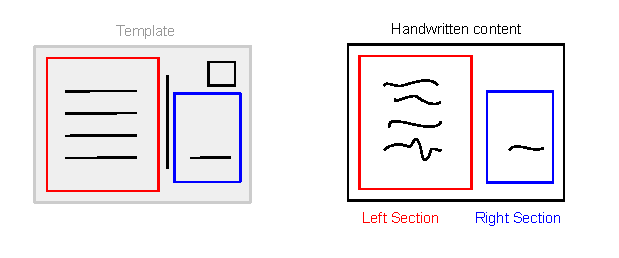
\includegraphics[trim={0cm 0cm 0 0cm}, width=1\textwidth]{./Chapter5/Figures/Main Sections Postcard}
	\caption{Postcard Main Sections}
	\label{fig:PFBoxes}
\end{figure}

\newpage

The ordering algorithm works like this:

We start by calculating the height of every box, using vector calculation. We do this for every box and divide by the number of boxes obtaining the average box height.

\begin{figure}[!ht]
	\centering
	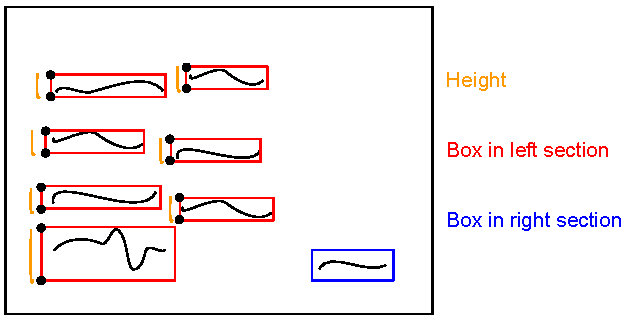
\includegraphics[trim={0cm -0.5cm 0 -0.5cm}, width=0.7\textwidth]{./Chapter5/Figures/Height Box}
	\caption{Average height calculation for left section}
	\label{fig:AVGH}
\end{figure}


Now all we have to do is pick the same located point in every box (top left or right left, etc...) and test the y value +- the calculated average box/2. If the y value is inside the range y-average height/2 to y+average height/2 then compare the x values else compare the y values. A lower x value means it comes earlier in the natural ordering. A higher y value than the current one means it comes later in the natural ordering. 

\section{Limitations}
IAM dataset vocabulary is primarily focused on the English language. It includes a wide range of alphanumeric characters, including uppercase and lowercase letters (A-Z, a-z), digits (0-9), and common punctuation marks. However, it does not cover the entire spectrum of possible characters that can exist in different languages or writing systems.

This vocabulary limitation means that the IAM dataset may not be suitable for recognizing text in languages other than English or for dealing with specialized symbols or characters that are outside the dataset's predefined set. For example, if the dataset does not include characters specific to a particular language or domain, the \gls{htr} model trained on IAM may struggle to accurately recognize and transcribe such characters.

While having made all the possible optimizations for using the detector, if the user draws text right next to each other there's a good change it will detect it all as a whole word.

\section{Results}
Results tend to vary a lot depending on the input image. 

Thicker line strokes, angled letters and image quality are some of the factors that directly influence the final output.

Higher quality images (more pixels) and thinner stroke lines tend to get better results.

These are the obtained results:
\begin{itemize}
	\item Figure~\ref{fig:T1} - Thiss is a tost image with arial font Hollo MHTPR model
	\item Figure~\ref{fig:T2} - Heito Worild Thiss is a HT. modet DoRs It works Antonio Canvatho
	\item Figure~\ref{fig:T3} - This is a tost Mello world Can you read thist 
	\item Figure~\ref{fig:T4} - this is a Tasst
\end{itemize} 

\begin{figure}[!ht]
	\centering
	\fbox{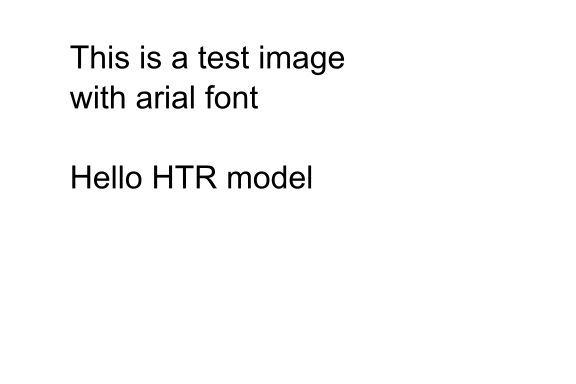
\includegraphics[trim={0cm -0.5cm 0 -0.5cm}, width=0.7\textwidth]{./Chapter5/Figures/test1}}
	\caption{Test figure 1}
	\label{fig:T1}
\end{figure}

\begin{figure}[!ht]
	\centering
	\fbox{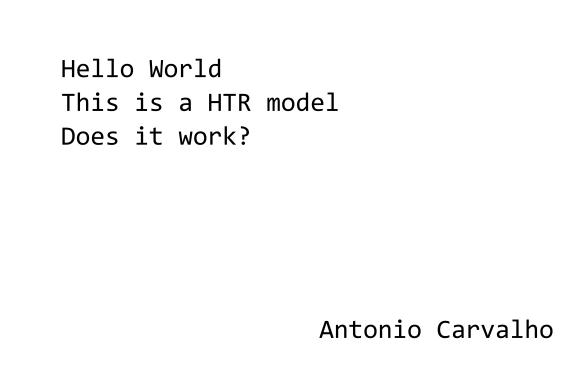
\includegraphics[trim={0cm -0.5cm 0 -0.5cm}, width=0.7\textwidth]{./Chapter5/Figures/test2}}
	\caption{Test figure 2}
	\label{fig:T2}
\end{figure}


\begin{figure}[!ht]
	\centering
	\fbox{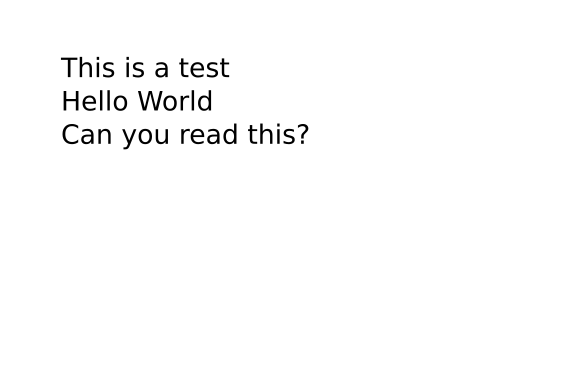
\includegraphics[trim={0cm -0.5cm 0 -0.5cm}, width=0.7\textwidth]{./Chapter5/Figures/test3}}
	\caption{Test figure 3}
	\label{fig:T3}
\end{figure}


\begin{figure}[!ht]
	\centering
	\fbox{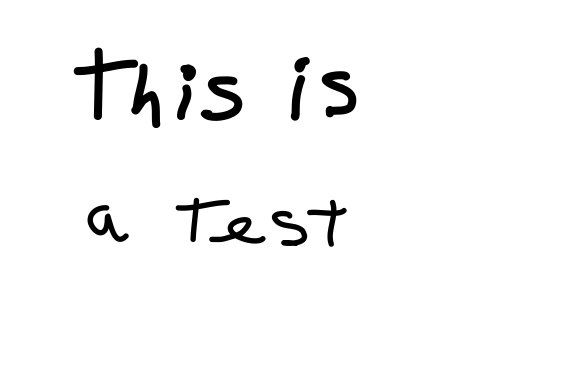
\includegraphics[trim={0cm -0.5cm 0 -0.5cm}, width=0.7\textwidth]{./Chapter5/Figures/test4}}
	\caption{Test figure 4}
	\label{fig:T4}
\end{figure}



